\documentclass[article]{jss}
\usepackage[utf8]{inputenc}

% jss.cls ----------------------------------------------------------------------

%% almost as usual
\author{Hadley Wickham\\RStudio}
\title{Tidy Data}

\Plainauthor{Hadley Wickham}
\Plaintitle{Tidy Data}

%% an abstract and keywords
\Abstract{
A huge amount of effort is spent cleaning data to get it ready for data analysis, but there has been little research on how to make data cleaning as easy and effective as possible. This paper tackles a small, but important, component of data cleaning: data ``tidying''. Tidy datasets are easy to manipulate, model and visualise, and have a specific structure: each variable is a column, each observation is a row, and each type of observational unit is a table. This framework makes it easy to tidy messy datasets because only a small set of tools are needed to deal with a wide range of un-tidy datasets. This structure also makes it easier to develop tidy tools for data analysis, tools that both input and output tidy datasets. The advantages of a consistent data structure and matching tools are demonstrated with a case study free from mundane data manipulation chores.
}
\Keywords{data cleaning, data tidying, relational databases, \proglang{R}}
\Plainkeywords{data cleaning, data tidying, relational databases, R}

%% \Volume{50}
%% \Issue{9}
%% \Month{June}
%% \Year{2012}
%% \Submitdate{2012-06-04}
%% \Acceptdate{2012-06-04}

\Address{
  Hadley Wickham\\
  Chief Scientist, RStudio\\
  Adjunct Professor, Rice University\\
  E-mail: \email{h.wickham@gmail.com}\\
  URL: \url{http://had.co.nz}
}

% jss.cls ----------------------------------------------------------------------

\DeclareGraphicsExtensions{.png,.pdf,.jpg}
\usepackage[format=plain,font=small]{caption}
\usepackage{booktabs}
\usepackage{fancyvrb}
\renewcommand{\FancyVerbFormatLine}[1]{R> #1}
\usepackage{epigraph}
\usepackage[subrefformat=parens]{subfig}

\begin{document}
\maketitle

\section{Introduction}

It's often said that 80\% of the effort in a data analysis is spent on data cleaning \citep{dasu:2003}, the process of getting the data ready to analyse. Data cleaning is not only a vital first step, but it is often repeated multiple times over the course of an analysis as new problems come to light. Despite the amount of time it takes, there has been little research on how to clean data well. Part of the challenge is the breadth of activities that cleaning encompasses, from outlier checking, to date parsing, to missing value imputation. To get a handle on the problem, this paper focusses on a small, but important, subset of data cleaning that I call data ``tidying'': structuring data values to make the process of data analysis as easy as possible.

The principles of tidy data provide a standard way of organising the data values within a dataset. A standard makes initial data cleaning easier because you don't need to start from scratch each time and you can avoid reinventing the wheel. The tidy data standard has been designed to facilitate initial exploration and analysis of the data, and it makes it easier to develop data analysis tools that work together seamlessly. Current tools are often inconsistent, so you need to spend time munging the output from one tool into the input for another. Tidy datasets and tidy tools work hand in hand to make data analysis easier, allowing you to focus on the interesting domain problem, not the uninteresting logistics of your data.

The principles of tidy data are closely tied to relational databases and Codd's relational algebra \citep{codd:1990}, but are framed in a language more familiar to statisticians. Computer scientists have also contributed much to the study of data cleaning. For example, \citet{lakshmanan:1996} defines an extension to SQL allowing it to operate on messy datasets, \citet{raman:2001} provides a framework for cleaning datasets, and \citet{kandel:2011} develops an interactive tool that makes data cleaning easy, automatically creating the code to clean datasets with a friendly user interface. These tools are useful, but they are presented in a language foreign to most statisticians, they fail to give much advice on how datasets should be structured, and they lack connections to the tools of data analysis.

The development of tidy data has been driven by my struggles working with real-world datasets, which are often organised in bizarre ways. I have spent countless hours struggling to get these datasets organised in a way that makes data analysis possible, let alone easy. I have also struggled to impart these skills to my students, so they can tackle problems in the real-world, where there are few constraints on how datasets are organised. In the course of these struggles I developed the \pkg{reshape} and \pkg{reshape2} \citep{wickham:2007b} \proglang{R} packages, but while I could intuitively use the tools, I lacked the framework to make my understanding explicit. This paper provides that framework, and provides a consistent ``philosophy of data'' that underlies my work in the \pkg{plyr} \citep{me:plyr} and \pkg{ggplot2} \citep{me:ggplot2} packages.

The paper proceeds as follows. Section~\ref{sec:defining} begins by defining the three characteristics that make a dataset tidy. Most real world datasets are not tidy, so Section~\ref{sec:tidying} describes the operations needed to make messy datasets tidy, and illustrates the techniques with a range of real examples. Section~\ref{sec:tidy-tools} defines tidy tools, tools that input and output tidy datasets, and discusses how together tidy data and tidy tools make it easier to do a data analysis. These principles are illustrated with a small case study in Section~\ref{sec:case-study}. Section~\ref{sec:discussion} concludes with a discussion of what this framework misses and what other approaches might be fruitful to pursue.

\section{Defining tidy data}
\label{sec:defining}

\epigraph{Happy families are all alike; every unhappy family is unhappy in its own way}{Leo Tolstoy}

Like families, tidy datasets are all alike, but every messy dataset is messy in its own way. Tidy datasets provide a standard way to connect the structure of a dataset (its physical layout) to its semantics (its meaning). I'll provide some standard vocabulary for describing the structure of a dataset, its semantics, and then use those definitions to define tidy data.

\subsection{Data structure}

Most statistical datasets are rectangular tables made up of \textbf{columns} and \textbf{rows}. The columns are almost always labelled, and rows are often labelled. Table~\ref{tbl:preg-raw-1} provides some data about an imaginary experiment in a format commonly seen in the wild. The table has two columns and three rows, and both rows and columns are labelled.

\begin{table}[htbp]
  \centering
  \begin{tabular}{lrr}
  \toprule
  & treatmenta & treatmentb \\ 
  \midrule
  John Smith & --- &   2 \\ 
  Jane Doe &  16 &  11 \\ 
  Mary Johnson &   3 &   1 \\ 
   \bottomrule
\end{tabular}

  \caption{Typical presentation dataset.}
  \label{tbl:preg-raw-1}
\end{table}

There are many ways to structure the same underlying data. Table~\ref{tbl:preg-raw-2} shows the same data as Table~\ref{tbl:preg-raw-1}, but the rows and columns have been transposed. The data is the same, but the layout is different. Our vocabulary of rows and columns is not rich enough to say why these two tables represent the same data. We also need a way to describe the meaning of the underlying data displayed in the table. It's not enough to describe the appearance of a dataset (how the values are physically laid out), we also need a way to describe the underlying semantics, the meaning, of the values in the dataset.

\begin{table}[htbp]
  \centering
  \begin{tabular}{lrrr}
  \toprule
  & John Smith & Jane Doe & Mary Johnson \\ 
  \midrule
  treatmenta & --- &  16 &   3 \\ 
  treatmentb &   2 &  11 &   1 \\ 
   \bottomrule
\end{tabular}

  \caption{The same data as in Table~\ref{tbl:preg-raw-1} but structured differently.}
  \label{tbl:preg-raw-2}
\end{table}

\subsection{Data semantics}

A table is a collection of data \textbf{values}, typically either numbers (if quantitative) or strings (if qualitative). Values are grouped into \textbf{variables}, measurements of a single quantifiable property. Multiple measurements made on the same observational unit form an \textbf{observation}. An observational unit is the smallest constituent atom of the experimental unit. For example, in a longitudinal medical study, the experimental unit might be the patient, but the observational unit is the patient at each time point. In an agricultural experiment, the experimental units might be the cages given different diets, but the observational units are the pigs whose individual weights are measured. This definition of observational unit leads to variables which are physical properties, like blood pressure and weight, not conditional properties like blood pressure at time 1, or weight of pig 2.

The dataset in Tables~\ref{tbl:preg-raw-1} and \ref{tbl:preg-raw-2} has three variables (name, treatment, result) and six observations (two for each person). It has two values of the treatment variable (a and b), three values of the treatment variable, and either five or six values of the result variable, depending on how you think about the missing value.  We can make this structure more obvious by putting the variables in the columns and the observations in the rows, as in Table~\ref{tbl:preg-tidy}.

\begin{table}[htbp]
  \centering
  \begin{tabular}{llr}
  \toprule
 name & trt & result \\ 
  \midrule
  John Smith & a & --- \\ 
  Jane Doe & a &  16 \\ 
  Mary Johnson & a &   3 \\ 
  John Smith & b &   2 \\ 
  Jane Doe & b &  11 \\ 
  Mary Johnson & b &   1 \\ 
   \bottomrule
\end{tabular}

  \caption{Tidied data.}
  \label{tbl:preg-tidy}
\end{table}

For a given dataset, it's usually easy to figure out what are observations and what are variables, but precisely defining variables and observations in general is surprisingly difficult. For example, if the columns in the Table~\ref{tbl:preg-raw-1} were height and weight we would have been happy to call them variables. If the columns were height and width, it would be less clear cut, as we might think of height and width as values of a dimension variable. If the columns were home phone and work phone, we could treat these as two variables, but in a fraud detection environment we might want variables phone number and number type because the use of one phone number for multiple people might suggest fraud. A general rule of thumb is that it is easier to describe functional relationships between variables (e.g., z is a linear combination of x and y, density is the ratio of weight to volume) than between rows, and it is easier to make comparisons between groups of observations (e.g., average of group a vs.\ average of group b) than between columns.

Note that in a given analysis, there may be multiple types of observational unit. For example, in a trial of new allergy medication we might have three observational types: demographic data collected from each person (age, sex, race), medical data collected from each person on each day (number of sneezes, redness of eyes), and meterological data collected on each day (temperature, pollen count).

\subsection{Tidy data}

Tidy data is a standard way of mapping the meaning of a dataset to its structure. A dataset is messy or tidy depending on how rows, columns and tables are matched up with observations, variables and types. In \textbf{tidy data}:

\begin{enumerate}
  \item Each variable forms a column,
  \item Each observation forms a row,
  \item Each type of observational unit forms a table.
\end{enumerate}

\noindent This is Codd's 3rd normal form \citep{codd:1990}, but with the constraints framed in statistical language, and the focus on a single dataset, not the many connected datasets common in relational databases. \textbf{Messy data} is any other other arrangement of the data. 

Table~\ref{tbl:preg-tidy} is the tidy version of Table~\ref{tbl:preg-raw-1} because each row represents an observation, the result of one treatment on one person, and each column is a variable. We could also choose to drop the row containing the missing value, because missing values should only be omitted if they are structural: impossible because of the design of the experiment.

Tidy data makes it easy for an analyst or a computer to extract needed variable because it provides a standard way of structuring a dataset. Contrast Table~\ref{tbl:preg-tidy} to Table~\ref{tbl:preg-raw-1}: in Table~\ref{tbl:preg-raw-1} you need to use different strategies for different variables. This slows analysis and invites errors. If you consider how many data analysis operations involve all of the values in a variable (every aggregating function), you can see how important it is to extract these values in a standard, simple way. Tidy data is particularly well suited for vectorised programming languages like \proglang{R}, because the layout ensures that values of different variables from the same observation are always paired.

While order of variables and observations does not affect analysis, a good ordering makes it easier to scan the raw values. One way of organising variables is by their role in the analysis: are values fixed by the design of the data collection, or are they measured during the course of the experiment? Fixed variables describe the experimental design and are known in advance. Computer scientists often call fixed variables dimensions, and statisticians usually denote them with subscripts on random variables. Measured variables are what we actually measure in the study. Fixed variables should come first, followed by measured variables, each ordered so that related variables are contiguous. Rows can then be ordered by the first variable, breaking ties with the second and subsequent (fixed) variables. This is the convention adopted by all tabular displays in this paper. 

\section{Tidying messy datasets}
\label{sec:tidying}

Real datasets can violate the three precepts of tidy data in almost every way imaginable, and often do. While occasionally you do get a dataset that you can start analysing immediately, this is the exception, not the norm.  This section describes the the five most common problems that make datasets messy, along with their remedies:

\begin{itemize}
  \item column headers are values, not variable names
  \item multiple variables are stored in one column
  \item variables are stored in both rows and columns
  \item multiple types of observational unit are stored in the same table
  \item a single observational unit is stored in multiple tables
\end{itemize}

Surprisingly, most messy datasets, including types of messiness not explicitly described above, can be tidied with a small set of tools: ``melting'', string splitting, and ``casting''. The following sections illustrate each problem with a real dataset that I have encountered in practice, and show how to tidy it. The complete datasets and the \proglang{R} code used to tidy them are available online at \url{https://github.com/hadley/tidy-data}, and in the online supplementary materials for this paper.

\subsection{Column headers are values, not variable names}

A common type of messy dataset is tabular data designed for presentation, where variables form both the rows and columns, and column headers are values, not variable names. While in this paper I call this arrangement messy, in some cases it can be extremely useful. It provides efficient storage for completely crossed designs, and it can provide extremely efficient computation if desired operations can be expressed as matrix operations. This issue is discussed in more depth in Section~\ref{sec:discussion}.

Table~\ref{tbl:pew-raw} shows a subset of a typical dataset of this form. This dataset explores the relationship between income and religion in the US, and comes from a report\footnote{\url{http://religions.pewforum.org/pdf/comparison-Income\%20Distribution\%20of\%20Religious\%20Traditions.pdf}} produced by the Pew Research Center. The Pew Center is an American think-tank that collects data on attitudes to topics ranging from religion to the internet, and produces many reports that contain datasets in the format shown.

\begin{table}[htbp]
  \centering
  % latex table generated in R 2.14.1 by xtable 1.6-0 package
% Mon Feb 13 11:37:03 2012
\begin{tabular}{lrrrrrrr}
  \toprule
 religion & $<$\$10k & \$10-20k & \$20-30k & \$30-40k & \$40-50k & \$50-75k & \$75-100k \\ 
  \midrule
  Agnostic &  27 &  34 &  60 &  81 &  76 & 137 & 122 \\ 
  Atheist &  12 &  27 &  37 &  52 &  35 &  70 &  73 \\ 
  Buddhist &  27 &  21 &  30 &  34 &  33 &  58 &  62 \\ 
  Catholic & 418 & 617 & 732 & 670 & 638 & 1116 & 949 \\ 
  Don’t know/refused &  15 &  14 &  15 &  11 &  10 &  35 &  21 \\ 
  Evangelical Prot & 575 & 869 & 1064 & 982 & 881 & 1486 & 949 \\ 
  Hindu &   1 &   9 &   7 &   9 &  11 &  34 &  47 \\ 
  Historically Black Prot & 228 & 244 & 236 & 238 & 197 & 223 & 131 \\ 
  Jehovah's Witness &  20 &  27 &  24 &  24 &  21 &  30 &  15 \\ 
  Jewish &  19 &  19 &  25 &  25 &  30 &  95 &  69 \\ 
   \bottomrule
\end{tabular}

  \caption{The first ten rows of data on income and religion from the Pew Forum. Two columns have been omitted to save space: `\$100-150k' and `\$150k'} 
  \label{tbl:pew-raw}
\end{table}

This dataset has three variables, religion, income and frequency, and to tidy it we need to ``melt'', or stack it, turning columns into rows. This makes ``wide'' datasets ``long'' or ``tall'', but I will avoid those terms because they are imprecise. Melting is parameterised by a list of columns that are already variables, or \textbf{colvar}s for short. The other columns are converted into two variables: a new ``column'' variable that contains repeated column headings and a ``value'' variable that contains a vector of data values concatenated from the previously separate columns. This is illustrated in Table~\ref{tbl:melt} with a toy dataset. The result of melting is a ``molten'' dataset.

\begin{table}
  \centering
  \subfloat[Raw data]{\label{tbl:melt-raw} \begin{tabular}{lrrr}
  \toprule
 row & a & b & c \\ 
  \midrule
  A &   1 &   4 &   7 \\ 
  B &   2 &   5 &   8 \\ 
  C &   3 &   6 &   9 \\ 
   \bottomrule
\end{tabular}
}%
  \hspace{2em}%
  \subfloat[Molten data]{\label{tbl:melt-molten}\begin{tabular}{llr}
  \toprule
 row & column & value \\ 
  \midrule
  A & a &   1 \\ 
  B & a &   2 \\ 
  C & a &   3 \\ 
  A & b &   4 \\ 
  B & b &   5 \\ 
  C & b &   6 \\ 
  A & c &   7 \\ 
  B & c &   8 \\ 
  C & c &   9 \\ 
   \bottomrule
\end{tabular}
}

  \caption{A simple example of melting. (a) is melted with one colvar, row, yielding the molten dataset (b). The information in each table is exactly the same, just stored in a different way.}
  \label{tbl:melt} 
\end{table}

The Pew dataset has one colvar, religion, and melting yields Table~\ref{tbl:pew-clean}. The column variable has been renamed to \code{income}, and the value column to \code{freq}, to better reflect their roles in this dataset. This form is tidy: each column represents a variable and each row represents an observation, in this case a demographic unit corresponding to a combination of religion and income.

\begin{table}[htbp]
  \centering
  % latex table generated in R 2.14.1 by xtable 1.6-0 package
% Mon Feb 13 11:37:03 2012
\begin{tabular}{llr}
  \toprule
 religion & income & freq \\ 
  \midrule
  Agnostic & $<$\$10k &  27 \\ 
  Agnostic & \$10-20k &  34 \\ 
  Agnostic & \$20-30k &  60 \\ 
  Agnostic & \$30-40k &  81 \\ 
  Agnostic & \$40-50k &  76 \\ 
  Agnostic & \$50-75k & 137 \\ 
  Agnostic & \$75-100k & 122 \\ 
  Agnostic & \$100-150k & 109 \\ 
  Agnostic & $>$150k &  84 \\ 
  Agnostic & Don't know/refused &  96 \\ 
   \bottomrule
\end{tabular}

  \caption{The first ten rows of the tidied Pew survey dataset on income and religion. The variable \code{column} has been renamed to income, and \code{value} to freq.}
  \label{tbl:pew-clean}
\end{table}

Another common use of this data format is to record regularly spaced observations over time. For example, the billboard dataset shown in Table~\ref{tbl:billboard-raw} records the date a song first entered the Billboard top 100. It has variables artist, track, date.entered, rank and week. The rank in each week after it enters the top 100 is recorded in 75 columns, \code{wk1} to \code{wk75}. If a song is in the top 100 for less than 75 weeks the remaining columns are filled with missing values.  This form of storage is not tidy, but is useful for data entry because it reduces duplication: otherwise each song in each week would need its own row, and song metadata like title and artist would need to be repeated. This issue will be discussed in more depth in Section~\ref{sub:multiple-types}.

\begin{table}[htbp]
  \centering
  % latex table generated in R 2.14.1 by xtable 1.6-0 package
% Wed Mar  7 06:59:34 2012
\begin{tabular}{rllllrrr}
  \toprule
 year & artist & track & time & date.entered & wk1 & wk2 & wk3 \\ 
  \midrule
  2000 & 2 Pac & Baby Don't Cry & 4:22 & 2000-02-26 &  87 &  82 &  72 \\ 
  2000 & 2Ge+her & The Hardest Part Of Breaking Up & 3:15 & 2000-09-02 &  91 &  87 &  92 \\ 
  2000 & 3 Doors Down & Kryptonite & 3:53 & 2000-04-08 &  81 &  70 &  68 \\ 
  2000 & 98° & Give Me Just One Night & 3:24 & 2000-08-19 &  51 &  39 &  34 \\ 
  2000 & A*Teens & Dancing Queen & 3:44 & 2000-07-08 &  97 &  97 &  96 \\ 
  2000 & Aaliyah & I Don't Wanna & 4:15 & 2000-01-29 &  84 &  62 &  51 \\ 
  2000 & Aaliyah & Try Again & 4:03 & 2000-03-18 &  59 &  53 &  38 \\ 
  2000 & Adams, Yolanda & Open My Heart & 5:30 & 2000-08-26 &  76 &  76 &  74 \\ 
   \bottomrule
\end{tabular}

  \caption{The first eight Billboard top hits for 2000. Other columns not shown are \code{wk4}, \code{wk5}, ..., \code{wk75}.}
  \label{tbl:billboard-raw}
\end{table}

This dataset has colvars year, artist, track, time, and date.entered. Melting yields Table~\ref{tbl:billboard-clean}. I have also done a little cleaning as well as tidying: the column variable has been converted to a week variable by extracting the week number, and I have added a date variable that combines the date the song entered the Billboard top 100 with the week number.

\begin{table}[htbp]
  \centering
  % latex table generated in R 2.14.1 by xtable 1.6-0 package
% Wed Mar  7 06:58:54 2012
\begin{tabular}{rllllrr}
  \toprule
 year & artist & time & track & date & week & rank \\ 
  \midrule
  2000 & 2 Pac & 4:22 & Baby Don't Cry & 2000-02-26 &   1 &  87 \\ 
  2000 & 2 Pac & 4:22 & Baby Don't Cry & 2000-03-04 &   2 &  82 \\ 
  2000 & 2 Pac & 4:22 & Baby Don't Cry & 2000-03-11 &   3 &  72 \\ 
  2000 & 2 Pac & 4:22 & Baby Don't Cry & 2000-03-18 &   4 &  77 \\ 
  2000 & 2 Pac & 4:22 & Baby Don't Cry & 2000-03-25 &   5 &  87 \\ 
  2000 & 2 Pac & 4:22 & Baby Don't Cry & 2000-04-01 &   6 &  94 \\ 
  2000 & 2 Pac & 4:22 & Baby Don't Cry & 2000-04-08 &   7 &  99 \\ 
  2000 & 2Ge+her & 3:15 & The Hardest Part Of Breaking Up & 2000-09-02 &   1 &  91 \\ 
  2000 & 2Ge+her & 3:15 & The Hardest Part Of Breaking Up & 2000-09-09 &   2 &  87 \\ 
  2000 & 2Ge+her & 3:15 & The Hardest Part Of Breaking Up & 2000-09-16 &   3 &  92 \\ 
  2000 & 3 Doors Down & 3:53 & Kryptonite & 2000-04-08 &   1 &  81 \\ 
  2000 & 3 Doors Down & 3:53 & Kryptonite & 2000-04-15 &   2 &  70 \\ 
  2000 & 3 Doors Down & 3:53 & Kryptonite & 2000-04-22 &   3 &  68 \\ 
  2000 & 3 Doors Down & 3:53 & Kryptonite & 2000-04-29 &   4 &  67 \\ 
  2000 & 3 Doors Down & 3:53 & Kryptonite & 2000-05-06 &   5 &  66 \\ 
   \bottomrule
\end{tabular}

  \caption{First fifteen rows of the tidied billboard dataset. The \code{date} column does not appear in the original table, but can be computed from \code{date.entered} and \code{week}.}
  \label{tbl:billboard-clean}
\end{table}

\subsection{Multiple variables stored in one column}

After melting, it often happens that the ``column'' variable is a combination of multiple underlying variables. This is illustrated by the tuberculosis (TB) dataset, a sample of which is shown in Table~\ref{tbl:tb-raw}. This dataset comes from the World Health Organisation, and records the counts of confirmed tuberculosis cases by country, year, and demographic group. The demographic groups are broken down by sex (m, f) and age (0--14, 15--25, 25--34, 35--44, 45--54, 55--64, unknown). 

\begin{table}[htbp]
  \centering
  % latex table generated in R 2.14.1 by xtable 1.6-0 package
% Wed Mar  7 07:12:31 2012
\begin{tabular}{lrrrrrrrrrr}
  \toprule
 country & year & m014 & m1524 & m2534 & m3544 & m4554 & m5564 & m65 & mu & f014 \\ 
  \midrule
  AD & 2000 &   0 &   0 &   1 &   0 &   0 &   0 &   0 & --- & --- \\ 
  AE & 2000 &   2 &   4 &   4 &   6 &   5 &  12 &  10 & --- &   3 \\ 
  AF & 2000 &  52 & 228 & 183 & 149 & 129 &  94 &  80 & --- &  93 \\ 
  AG & 2000 &   0 &   0 &   0 &   0 &   0 &   0 &   1 & --- &   1 \\ 
  AL & 2000 &   2 &  19 &  21 &  14 &  24 &  19 &  16 & --- &   3 \\ 
  AM & 2000 &   2 & 152 & 130 & 131 &  63 &  26 &  21 & --- &   1 \\ 
  AN & 2000 &   0 &   0 &   1 &   2 &   0 &   0 &   0 & --- &   0 \\ 
  AO & 2000 & 186 & 999 & 1003 & 912 & 482 & 312 & 194 & --- & 247 \\ 
  AR & 2000 &  97 & 278 & 594 & 402 & 419 & 368 & 330 & --- & 121 \\ 
  AS & 2000 & --- & --- & --- & --- &   1 &   1 & --- & --- & --- \\ 
   \bottomrule
\end{tabular}

  \caption{Original TB dataset. Corresponding to each `m' column for males, there is also an `f' column for females: \code{f1524}, \code{f2534} and so on. These are not shown to conserve space. Note the mixture of 0s and missing values (---): this is due to the data collection process and the distinction is important for this dataset.}
  \label{tbl:tb-raw}
\end{table}

Column headers in this format are often separated by some character (\code{.}, \code{-}, \code{\_}, \code{:}) and the string can be broken into pieces using that character as a divider. In other cases, such as for this dataset, more careful string processing is required, or the variable names need to be matched to a lookup table that converts single compound values to values of multiple variables. 

Table~\subref*{tbl:tb-molten} shows the results of melting the TB dataset, and Table~\subref*{tbl:tb-tidy} the results of splitting the column ``column'' into two real variables: age and sex.  

\begin{table}[htbp]
  \centering
  \subfloat[Molten data]{\label{tbl:tb-molten}% latex table generated in R 2.14.1 by xtable 1.6-0 package
% Wed Mar  7 07:12:31 2012
\begin{tabular}{lrlr}
  \toprule
 country & year & column & cases \\ 
  \midrule
  AD & 2000 & m014 &   0 \\ 
  AD & 2000 & m1524 &   0 \\ 
  AD & 2000 & m2534 &   1 \\ 
  AD & 2000 & m3544 &   0 \\ 
  AD & 2000 & m4554 &   0 \\ 
  AD & 2000 & m5564 &   0 \\ 
  AD & 2000 & m65 &   0 \\ 
  AE & 2000 & m014 &   2 \\ 
  AE & 2000 & m1524 &   4 \\ 
  AE & 2000 & m2534 &   4 \\ 
  AE & 2000 & m3544 &   6 \\ 
  AE & 2000 & m4554 &   5 \\ 
  AE & 2000 & m5564 &  12 \\ 
  AE & 2000 & m65 &  10 \\ 
  AE & 2000 & f014 &   3 \\ 
   \bottomrule
\end{tabular}
}%
  \hspace{2em}%
  \subfloat[Tidy data]{\label{tbl:tb-tidy}% latex table generated in R 2.14.1 by xtable 1.6-0 package
% Wed Mar  7 07:12:31 2012
\begin{tabular}{lrllr}
  \toprule
 country & year & sex & age & cases \\ 
  \midrule
  AD & 2000 & m & 0-14 &   0 \\ 
  AD & 2000 & m & 15-24 &   0 \\ 
  AD & 2000 & m & 25-34 &   1 \\ 
  AD & 2000 & m & 35-44 &   0 \\ 
  AD & 2000 & m & 45-54 &   0 \\ 
  AD & 2000 & m & 55-64 &   0 \\ 
  AD & 2000 & m & 65+ &   0 \\ 
  AE & 2000 & m & 0-14 &   2 \\ 
  AE & 2000 & m & 15-24 &   4 \\ 
  AE & 2000 & m & 25-34 &   4 \\ 
  AE & 2000 & m & 35-44 &   6 \\ 
  AE & 2000 & m & 45-54 &   5 \\ 
  AE & 2000 & m & 55-64 &  12 \\ 
  AE & 2000 & m & 65+ &  10 \\ 
  AE & 2000 & f & 0-14 &   3 \\ 
   \bottomrule
\end{tabular}
}
  
  \caption{Tidying the TB dataset requires first melting, and then splitting the ``column'' column into two variables: sex and age.}
  \label{tbl:tb-clean}
\end{table}

Storing the values in this form resolves another problem in the original data: we want to compare rates, not counts, but to compute rates we need to know the population. In the original format, there is no easy way to add a population variable, and it has to be stored in a separate table, which makes it hard to correctly match populations to counts. In tidy form, adding variables to store population and rate is easy: they just become additional columns.

\subsection{Variables are stored in both rows and columns}

The most complicated form of messy data is when variables have been stored in both rows and columns. Table~\ref{tbl:weather-raw} shows daily weather data from the Global Historical Climatology Network for one weather station (MX17004) in Mexico for five months in 2010. It has variables in individual columns (id, year, month), spread across columns (day, d1--d31) and across rows (tmin, tmax) (minimum and maximum temperature). Months with less than 31 days have structural missing values for the last day(s) of the month. The element column is not a variable: it stores the names of variables.

To tidy this dataset we first melt it with colvars id, year, month and the column that contains variable names, element, yielding Table~\subref*{tbl:weather-molten}. For presentation, we have dropped the missing values, making them implicit rather than explicit. This is permissible because we know how many days are in each month and can easily reconstruct the explicit missing values.

This dataset is mostly tidy, but we have two variables stored in rows: \code{tmin} and \code{tmax}, the type of observation. Not shown in this example are other meteorological variables prcp (precipitation) and snow (snowfall). Fixing this requires the cast, or unstack, operation, which performs the inverse of melting, rotating the \code{element} variable back out into the columns to give Table~\subref*{tbl:weather-tidy}. This form is tidy: there is one variable in each column, and each row represents a day's observations. The cast operation is described in depth in \citet{wickham:2007b}.

\begin{table}[htbp]
  \centering
  \begin{tabular}{lrrlrrrrrrrr}
  \toprule
 id & year & month & element & d1 & d2 & d3 & d4 & d5 & d6 & d7 & d8 \\ 
  \midrule
  MX17004 & 2010 &  1 & tmax & --- & --- & --- & --- & --- & --- & --- & --- \\ 
  MX17004 & 2010 &  1 & tmin & --- & --- & --- & --- & --- & --- & --- & --- \\ 
  MX17004 & 2010 &  2 & tmax & --- & 27.3 & 24.1 & --- & --- & --- & --- & --- \\ 
  MX17004 & 2010 &  2 & tmin & --- & 14.4 & 14.4 & --- & --- & --- & --- & --- \\ 
  MX17004 & 2010 &  3 & tmax & --- & --- & --- & --- & 32.1 & --- & --- & --- \\ 
  MX17004 & 2010 &  3 & tmin & --- & --- & --- & --- & 14.2 & --- & --- & --- \\ 
  MX17004 & 2010 &  4 & tmax & --- & --- & --- & --- & --- & --- & --- & --- \\ 
  MX17004 & 2010 &  4 & tmin & --- & --- & --- & --- & --- & --- & --- & --- \\ 
  MX17004 & 2010 &  5 & tmax & --- & --- & --- & --- & --- & --- & --- & --- \\ 
  MX17004 & 2010 &  5 & tmin & --- & --- & --- & --- & --- & --- & --- & --- \\ 
   \bottomrule
\end{tabular}

  \caption{Original weather dataset.  There is a column for each possible day in the month.  Columns \code{d11} to \code{d31} have been omitted to conserve space.}
  \label{tbl:weather-raw}
\end{table}

\begin{table}[htbp]
  \centering
  \subfloat[Molten data]%
    {\label{tbl:weather-molten}\begin{tabular}{lllr}
  \toprule
 id & date & element & value \\ 
  \midrule
  MX17004 & 2010-01-30 & tmax & 27.8 \\ 
  MX17004 & 2010-01-30 & tmin & 14.5 \\ 
  MX17004 & 2010-02-02 & tmax & 27.3 \\ 
  MX17004 & 2010-02-02 & tmin & 14.4 \\ 
  MX17004 & 2010-02-03 & tmax & 24.1 \\ 
  MX17004 & 2010-02-03 & tmin & 14.4 \\ 
  MX17004 & 2010-02-11 & tmax & 29.7 \\ 
  MX17004 & 2010-02-11 & tmin & 13.4 \\ 
  MX17004 & 2010-02-23 & tmax & 29.9 \\ 
  MX17004 & 2010-02-23 & tmin & 10.7 \\ 
   \bottomrule
\end{tabular}
}%
  \hspace{2em}%
  \subfloat[Tidy data]%
    {\label{tbl:weather-tidy}\begin{tabular}{llrr}
  \toprule
 id & date & tmax & tmin \\ 
  \midrule
  MX17004 & 2010-01-30 & 27.8 & 14.5 \\ 
  MX17004 & 2010-02-02 & 27.3 & 14.4 \\ 
  MX17004 & 2010-02-03 & 24.1 & 14.4 \\ 
  MX17004 & 2010-02-11 & 29.7 & 13.4 \\ 
  MX17004 & 2010-02-23 & 29.9 & 10.7 \\ 
  MX17004 & 2010-03-05 & 32.1 & 14.2 \\ 
  MX17004 & 2010-03-10 & 34.5 & 16.8 \\ 
  MX17004 & 2010-03-16 & 31.1 & 17.6 \\ 
  MX17004 & 2010-04-27 & 36.3 & 16.7 \\ 
  MX17004 & 2010-05-27 & 33.2 & 18.2 \\ 
   \bottomrule
\end{tabular}
}%

  \caption{(a) Molten weather dataset.  This is almost tidy, but the \code{element} column contains names of variables, not values. Missing values are dropped to conserve space. (b) Tidy weather dataset. Each row represents the meteorological measurements for a single day.  There are two measured variables, minimum (\code{tmin}) and maximum (\code{tmax}) temperature; all other variables are fixed.}
  \label{tbl:weather-clean}
\end{table}

\subsection{Multiple types in one table}
\label{sub:multiple-types}

Datasets often involve values collected at multiple levels, on different types of observational unit. During tidying, each type of observational unit should be stored in its own table. This is closely related to the idea of database normalisation, where each fact is expressed in only one place; if not, it's possible for inconsistencies to occur. 

%If you're not familiar with normalisation, it can be worthwhile to learn a little about it. There are many good tutorials available online - I found \url{http://phlonx.com/resources/nf3/} after a few minutes of searching. You certainly don't need to become an expert, as most statistical databases only need a small amount of normalisation, but it is extremely helpful for identifying inconsistencies in your data.

The billboard dataset described in Table~\ref{tbl:billboard-clean} actually contains observations on two types of observational unit: the song, and its rank in each week. This is revealed through the duplication of facts about the song: the artist and time are repeated for every song in each week. The billboard dataset needs to be broken down into two datasets: a song dataset which stores artist, song name and time; and a ranking dataset which gives the rank of the song in each week. Table~\ref{tbl:billboard-normal} shows these two datasets. You could also imagine a week dataset which would record background information about the week, maybe the total number of songs sold or similar ``demographic'' information.

\begin{table}
  \centering
  % latex table generated in R 2.14.1 by xtable 1.6-0 package
% Wed Mar  7 06:58:54 2012
\begin{tabular}{rlll}
  \toprule
 id & artist & track & time \\ 
  \midrule
    1 & 2 Pac & Baby Don't Cry & 4:22 \\ 
    2 & 2Ge+her & The Hardest Part Of Breaking Up & 3:15 \\ 
    3 & 3 Doors Down & Kryptonite & 3:53 \\ 
    4 & 3 Doors Down & Loser & 4:24 \\ 
    5 & 504 Boyz & Wobble Wobble & 3:35 \\ 
    6 & 98° & Give Me Just One Night & 3:24 \\ 
    7 & A*Teens & Dancing Queen & 3:44 \\ 
    8 & Aaliyah & I Don't Wanna & 4:15 \\ 
    9 & Aaliyah & Try Again & 4:03 \\ 
   10 & Adams, Yolanda & Open My Heart & 5:30 \\ 
   11 & Adkins, Trace & More & 3:05 \\ 
   12 & Aguilera, Christina & Come On Over Baby & 3:38 \\ 
   13 & Aguilera, Christina & I Turn To You & 4:00 \\ 
   14 & Aguilera, Christina & What A Girl Wants & 3:18 \\ 
   15 & Alice Deejay & Better Off Alone & 6:50 \\ 
   \bottomrule
\end{tabular}
\hspace{1em}%
  \begin{tabular}{rlr}
  \toprule
 id & date & rank \\ 
  \midrule
    1 & 2000-02-26 &  87 \\ 
    1 & 2000-03-04 &  82 \\ 
    1 & 2000-03-11 &  72 \\ 
    1 & 2000-03-18 &  77 \\ 
    1 & 2000-03-25 &  87 \\ 
    1 & 2000-04-01 &  94 \\ 
    1 & 2000-04-08 &  99 \\ 
    2 & 2000-09-02 &  91 \\ 
    2 & 2000-09-09 &  87 \\ 
    2 & 2000-09-16 &  92 \\ 
    3 & 2000-04-08 &  81 \\ 
    3 & 2000-04-15 &  70 \\ 
    3 & 2000-04-22 &  68 \\ 
    3 & 2000-04-29 &  67 \\ 
    3 & 2000-05-06 &  66 \\ 
   \bottomrule
\end{tabular}


  \caption{Normalised billboard dataset split up into song dataset (left) and rank dataset (right). First 15 rows of each dataset shown; \code{genre} omitted from song dataset, \code{week} omitted from rank dataset.}
  \label{tbl:billboard-normal}
\end{table}

Normalisation is useful for tidying and eliminating inconsistencies, but there are few data analysis tools that work directly with relational data, so analysis usually requires denormalisation, merging the datasets back into one table. 

% Multiple-choice/check all that apply data

\subsection{One type in multiple tables}

It's also common to find data values about a single type of observational unit spread out over multiple tables, or multiple files. These tables are often split up by another variable, so each file represents a single year, person, or location. As long as the format for individual records is consistent, this is an easy problem to fix: 

\begin{enumerate}
  \item read the files into a list of tables,

\item for each table, add a new column that records the original file name (because the file name is often the value of an important variable), then

  \item combine all tables into a single table. 
\end{enumerate}

Once you have a single table, you can perform additional tidying as needed. An example of this type of cleaning can be found at \url{https://github.com/hadley/data-baby-names} which takes 129 yearly baby name tables provided by the US Social Security Administration and combines them into a single file.

A more complicated situation occurs when the dataset structure has changed over time. For example, the datasets contain different variables, the same variables have different names, different file formats are used, or there are different conventions for missing values. This may require each file to tidied individually (or, if you're lucky, in small groups) and then combined once tidied. An example of this type of tidying is illustrated in \url{https://github.com/hadley/data-fuel-economy}, which shows the tidying of {\sc epa} fuel economy data for over 50,000 cars from 1978 to 2008. The raw data is available online, but each year is stored in a separate file and there are four major formats with many minor variations, making tidying this dataset a considerable challenge.

\section{Tidy tools}
\label{sec:tidy-tools}

Once you have a tidy dataset, what can you do with it? Tidy data is only worthwhile if it makes analysis easier. This section discusses tidy tools, tools that take tidy datasets as input and return tidy datasets as output. Tidy tools are useful because the output of one tool can be used as the input to another, making it straightforward to compose multiple tools to solve a problem. Tidy data also ensures that variables are stored in a consistent, explicit manner. This makes each tool simpler, because it doesn't need a Swiss Army knife of parameters for dealing with different dataset structures.

Tools can be messy for two reasons: either they take messy datasets as input (messy-input tools) or they produce messy datasets as output (messy-output tools). Messy-input tools are typically more complicated than tidy-input tools because they need to include some parts of the tidying process. This can be useful for common types of messy datasets, but it typically makes the function more complex, harder to use and harder to maintain. Messy-output tools are frustrating and slow down analysis because they can not be easily composed and you must constantly think about how to convert from one format to another. We'll see examples of both in the following sections.

Next, I give examples of tidy and messy tools for three important components of analysis: data manipulation, visualisation and modelling. I will focus particularly on tools provided by \proglang{R} \citep{R}, because it has many existing tidy tools, but I will also touch on other statistical programming environments.

\subsection{Manipulation}

Data manipulation includes variable-by-variable transformation (e.g., \code{log} or \code{sqrt}), as well as aggregation, filtering and reordering. In my experience, there are four extremely common operations that are performed over and over again in the course of an analysis. These are the four fundamental verbs of data manipulation:

\begin{itemize}

  \item Filtering, or subsetting, where observations are removed based on some
  condition.

  \item Transforming, where new variables are added or existing variables
  modified. These modifications can involve either a single variable (e.g., 
  log-transforming a variable), or involve multiple variables (e.g., computing
  density from weight and volume).

  \item Aggregating, where multiple values are collapsed into a single value,
  e.g., by summing or taking means.

  \item Sorting, where the order of observations is changed.

\end{itemize}

All these operations are made easier when there is a consistent way to refer to variables. Tidy data provides this because each variable lives in its own column.

In \proglang{R}, filtering and transforming are performed by the base \proglang{R} functions \code{subset} and \code{transform}. These are input and output-tidy. The \code{aggregate} function performs group-wise aggregation, is input-tidy, and is output-tidy providing a single aggregation method is used. The \pkg{plyr} package provides a tidy \code{summarise} and \code{arrange} function for aggregation and sorting.

The four verbs can be, and often are, modified by the ``by'' preposition. We often need group-wise aggregates, transformations or subsets: pick the biggest in each group, average over replicates and so on. Combining each of the four verbs with a by operator allows them to operate on subsets of a data frame at a time. Many \proglang{SAS} {\sc proc}s possess a {\sc by} statement which allows the operation to be performed by group, and are generally input-tidy. Base \proglang{R} possesses a \code{by} function, which is input-tidy, but not output-tidy, because it produces a list. The \code{ddply} function from the \pkg{plyr} package is a tidy alternative.

% Some aggregations occur so frequently they deserve their own optimised implementations. One such operation is (weighted) counting. Base R provides the {\tt table} function for this, but it is not output-tidy: it returns a multidimensional array. An tidy alternative is the {\tt count} function from {\tt plyr}, which returns a tidy dataset with a column for each of the input variables plus a new variable {\tt freq}, which records the number of records in each category.

Other tools are needed when we have multiple datasets. An advantage of tidy data is the ease with which it can be combined with other tidy datasets: we just need a join operator which works by matching common variables and adding new columns. This is implemented in the \code{merge} function in base \proglang{R}, or the \code{join} function in \pkg{plyr}. Compare this to the difficulty of combining datasets stored in arrays; these typically require painstaking alignment before matrix operations can be used, and errors can be very hard to detect.

\subsection{Visualisation}

Tidy visualisation tools only need to be input-tidy as their output is visual. Domain specific languages work particularly well for the visualisation of tidy datasets because they can describe a visualisation as a mapping between variables in the dataset and aesthetic properties of the graphic like position, size, shape and colour. This is the idea behind the grammar of graphics \citep{wilkinson:2006}, and the layered grammar of graphics \citep{wickham:2007d}, an extension tailored specifically for \proglang{R}.

Most graphical tools in \proglang{R} are input tidy, including the \pkg{base} \code{plot} function, the \pkg{lattice} family of plots \citep{sarkar:2008} and \pkg{ggplot2} \citep{me:ggplot2}. Some specialised tools exist for visualising messy datasets. Some base \proglang{R} functions like \code{barplot}, \code{matplot}, \code{dotchart}, and \code{mosaicplot}, work with messy datasets where variables are spread out over multiple columns. Similarly, the parallel coordinates plot \citep{wegman:1990,inselberg:1985} can be used to create time series plots for messy datasets where each time point is a column.

\subsection{Modelling}
\label{sub:modelling}

Modelling is the inspiration that has driven much of this work, because most modelling tools work best with tidy datasets. Every statistical language has a way of describing a model as a connection between different variables, a domain specific language that connects responses to predictors: 

\begin{itemize}

  \item \proglang{R} (\code{lm}): \code{y ~ a + b + c * d}

  \item \proglang{SAS} (\code{PROC GLM}): \code{y = a + b + c * d}

  \item \proglang{SPSS} (\code{glm}): \code{y BY a b c d / DESIGN a b c d c * d}

  \item \proglang{Stata} (\code{regress}): \code{y a b c \# d}


\end{itemize}

This is not to say that tidy data is the format used internally to compute the regression. Significant transformations take place to produce a numeric matrix that can easily be fed to standard linear algebra routines. Common transformations include adding an intercept column (column of all ones), turning categorical variables into multiple binary dummy variables, and for smooth terms like splines, projecting the data values on to the appropriate basis functions.

% http://support.sas.com/documentation/cdl/en/statug/63033/HTML/default/viewer.htm#statug_glm_sect022.htm

There have been some attempts to adapt modelling functions for specific types of messy datasets. For example, in \proglang{SAS}'s \code{proc glm}, multiple variables on the response side of the equation will be interpreted as repeated measures if the {\sc repeated} keyword is present. For the raw billboard data, we could construct a model of the form \code{wk1-wk76 = track} instead of \code{rank = week * track} on the tidy data (provided week is labelled as a categorical variable). 

Another interesting example is the classic paired t-test, which can be computed in two ways depending on how the data is stored. If the data is stored as in Table~\subref*{tbl:paired}, then a paired t-test is just a t-test applied to the mean difference between x and y. If it is stored in the form of Table~\subref*{tbl:mixed}, then an equivalent model is to fit a mixed effects model, with a fixed dummy variable representing the ``variable'', and a random intercept for each id. (In \proglang{R}'s lmer4 notation, this is \code{value ~ variable + (1 | id)}). Either way of modelling the data yields the same result. Without more information we can't say which form of the data is tidy: if x and y represent length of left and right arms, then Table~\subref*{tbl:paired} is tidy, if x and y represent measurements on day 1 and day 10, then Table~\subref*{tbl:mixed} is tidy.

\begin{table}
  \centering
  \subfloat[Data for paired t-test]{
    \label{tbl:paired}
    % latex table generated in R 2.14.2 by xtable 1.6-0 package
% Wed Mar 21 10:40:47 2012
\begin{tabular}{rrr}
  \toprule
 id & x & y \\ 
  \midrule
    1 & 22.19 & 24.05 \\ 
    2 & 19.82 & 22.91 \\ 
    3 & 19.81 & 21.19 \\ 
    4 & 17.49 & 18.59 \\ 
    5 & 19.44 & 19.85 \\ 
   \bottomrule
\end{tabular}

  }%
  \hspace{2em}%
  \subfloat[Data for mixed effects model]{
    \label{tbl:mixed}
    % latex table generated in R 2.14.2 by xtable 1.6-0 package
% Wed Mar 21 10:40:47 2012
\begin{tabular}{rlr}
  \toprule
 id & variable & value \\ 
  \midrule
    1 & x & 22.19 \\ 
    2 & x & 19.82 \\ 
    3 & x & 19.81 \\ 
    4 & x & 17.49 \\ 
    5 & x & 19.44 \\ 
    1 & y & 24.05 \\ 
    2 & y & 22.91 \\ 
    3 & y & 21.19 \\ 
    4 & y & 18.59 \\ 
    5 & y & 19.85 \\ 
   \bottomrule
\end{tabular}

  }

  \caption{Two data sets for performing the same test.}
  \label{label}
\end{table}

While model inputs usually require tidy inputs, model outputs, such as predictions and estimated coefficients, aren't always tidy. This makes it more difficult to combine results from multiple models. For example, in \proglang{R}, the default representation of model coefficients is not tidy because it does not have an explicit variable that records the variable name for each estimate: these are instead recorded as row names. In \proglang{R}, row names must be unique, so combining coefficients from many models (e.g., from bootstrap resamples, or subgroups) requires workarounds to avoid losing important information. This knocks you out of the flow of analysis and makes it harder to combine the results from multiple models.

\section{Case study} 
\label{sec:case-study}

The following case study illustrates how tidy data and tidy tools make data analysis easier by easing the transitions between manipulation, visualisation and modelling: you will not see any code that exists solely to get the output of one function into the right format for input to another. I'll show the \proglang{R} code that performs the analysis, but even if you're not familiar with \proglang{R} or the exact idioms I use, I've tried to make it easy to understand by tightly interleaving code, results and explanation.

The case study uses individual-level mortality data from Mexico, with the goal of finding causes of death that have notably different time patterns within a day. The full dataset has information on 539,530 deaths in Mexico in 2008 and 55 variables, including the the location and time of death, the cause of death, and demographics of the deceased. Table~\ref{fig:raw} shows a small sample of the dataset, focussing on variables related to time of death (year, month, day and hour), and cause (cod).

\begin{table}
  \centering
  \begin{tabular}{rrrrl}
  \toprule
 yod & mod & dod & hod & cod \\ 
  \midrule
  2008 &   1 &   1 &   1 & B20 \\ 
  2008 &   1 &   2 &   4 & I67 \\ 
  2008 &   1 &   3 &   8 & I50 \\ 
  2008 &   1 &   4 &  12 & I50 \\ 
  2008 &   1 &   5 &  16 & K70 \\ 
  2008 &   1 &   6 &  18 & I21 \\ 
  2008 &   1 &   7 &  20 & I21 \\ 
  2008 &   1 &   8 & --- & K74 \\ 
  2008 &   1 &  10 &   5 & K74 \\ 
  2008 &   1 &  11 &   9 & I21 \\ 
  2008 &   1 &  12 &  15 & I25 \\ 
  2008 &   1 &  13 &  20 & R54 \\ 
  2008 &   1 &  15 &   2 & I61 \\ 
  2008 &   1 &  16 &   7 & I21 \\ 
  2008 &   1 &  17 &  13 & I21 \\ 
   \bottomrule
\end{tabular}

  \caption{A sample of 16 rows and 5 columns from the original dataset of 539,530 rows and 55 columns.}
  \label{fig:raw}
\end{table}

To achieve our goal of finding unusual time courses, we'll start by counting the number of deaths in each hour (\code{hod}) for each cause (\code{cod}) with the tidy \code{count} function. Then we remove missing (and hence uninformative for our purpose) values with \code{subset}. This gives Table~\subref*{tbl:counts:1}.

First, we count the the number of deaths in each hour of the day for each cause of death, and remove missing observations:

\begin{Verbatim}
hod2 <- count(deaths, c("hod", "cod"))
hod2 <- subset(hod2, !is.na(hod))
\end{Verbatim}

Next we join the dataset to \code{codes} dataset that gives informative labels for the disease. These two datasets are connected by the \code{cod} variable. This adds a new variable, \code{disease}, shown in Table~\subref*{tbl:counts:2}).

\begin{Verbatim}
hod2 <- join(hod2, codes, by = "cod")
\end{Verbatim}

The total deaths for each cause vary over several orders of magnitude: there were 46,794 deaths from heart attack, and 10 deaths from avalanche. This means that it makes more sense to compare the proportion of deaths in each hour, rather than the total number. We compute this by breaking the dataset down by \code{cod}, and then \code{transform}ing to add a new \code{prop} column, the hourly frequency divided by the total number of deaths from that cause. This new columns is Table~\subref*{tbl:counts:3}.

\code{ddply} breaks down its first argument (\code{hod2}) by its second argument (the \code{cod} variable), and applies its third argument (\code{transform}) to each piece. The fourth argument (\code{prop = freq / sum(freq)}) is passed on to transform.

\begin{Verbatim}
hod2 <- ddply(hod2, "cod", transform, prop = freq / sum(freq))
\end{Verbatim}

We then compute the overall average death rate for each hour, and merge that back into the original dataset. This yields Table~\subref*{tbl:counts:4} and allows us to easily compare each disease with the overall pattern by comparing \code{prop} to \code{prop\_all}.


First, we work out the number of people dying each hour by breaking down \code{hod2} by \code{hod}, summarising with a total for over each cause of death.

\begin{Verbatim}
overall <- ddply(hod2, "hod", summarise, freq_all = sum(freq))
\end{Verbatim}

Next, we work out the overall proportion of people dying in each hour:

\begin{Verbatim}
overall <- transform(overall, prop_all = freq_all / sum(freq_all))
\end{Verbatim}

Then finally, we join the overall dataset with the individual dataset to make it easier to compare the two:

\begin{Verbatim}
hod2 <- join(hod2, overall, by = "hod")
\end{Verbatim}

\begin{table}[htbp]
  \centering
  \subfloat[]{
    \label{tbl:counts:1}\begin{tabular}{rlr}
  \toprule
 hod & cod & freq \\ 
  \midrule
    8 & B16 &   4 \\ 
    8 & E84 &   3 \\ 
    8 & I21 & 2205 \\ 
    8 & N18 & 315 \\ 
    9 & B16 &   7 \\ 
    9 & E84 &   1 \\ 
    9 & I21 & 2209 \\ 
    9 & N18 & 333 \\ 
   10 & B16 &  10 \\ 
   10 & E84 &   7 \\ 
   10 & I21 & 2434 \\ 
   10 & N18 & 343 \\ 
   11 & B16 &   6 \\ 
   11 & E84 &   3 \\ 
   11 & I21 & 2128 \\ 
   \bottomrule
\end{tabular}

  }%
  \subfloat[]{
    \label{tbl:counts:2}% latex table generated in R 2.14.2 by xtable 1.6-0 package
% Wed Apr  4 08:45:15 2012
\begin{tabular}{l}
  \toprule
 disease \\ 
  \midrule
  Acute hepatitis B \\ 
  Cystic fibrosis \\ 
  Acute myocardial infarction \\ 
  Chronic renal failure \\ 
  Acute hepatitis B \\ 
  Cystic fibrosis \\ 
  Acute myocardial infarction \\ 
  Chronic renal failure \\ 
  Acute hepatitis B \\ 
  Cystic fibrosis \\ 
  Acute myocardial infarction \\ 
  Chronic renal failure \\ 
  Acute hepatitis B \\ 
  Cystic fibrosis \\ 
  Acute myocardial infarction \\ 
   \bottomrule
\end{tabular}

  }%
  \subfloat[]{
    \label{tbl:counts:3}% latex table generated in R 2.14.2 by xtable 1.6-0 package
% Wed Apr  4 08:45:15 2012
\begin{tabular}{r}
  \toprule
 prop \\ 
  \midrule
  0.04 \\ 
  0.03 \\ 
  0.05 \\ 
  0.04 \\ 
  0.07 \\ 
  0.01 \\ 
  0.05 \\ 
  0.04 \\ 
  0.10 \\ 
  0.07 \\ 
  0.05 \\ 
  0.04 \\ 
  0.06 \\ 
  0.03 \\ 
  0.05 \\ 
   \bottomrule
\end{tabular}

  }%
  \subfloat[]{
    \label{tbl:counts:4}% latex table generated in R 2.14.2 by xtable 1.6-0 package
% Wed Apr  4 08:45:15 2012
\begin{tabular}{rr}
  \toprule
 freq\_all & prop\_all \\ 
  \midrule
  21915 & 0.04 \\ 
  21915 & 0.04 \\ 
  21915 & 0.04 \\ 
  21915 & 0.04 \\ 
  22401 & 0.04 \\ 
  22401 & 0.04 \\ 
  22401 & 0.04 \\ 
  22401 & 0.04 \\ 
  24321 & 0.05 \\ 
  24321 & 0.05 \\ 
  24321 & 0.05 \\ 
  24321 & 0.05 \\ 
  23843 & 0.05 \\ 
  23843 & 0.05 \\ 
  23843 & 0.05 \\ 
   \bottomrule
\end{tabular}

  }
  
  \caption{A sample of four diseases and four hours from \code{hod2} data frame.}
  \label{tbl:counts}
\end{table}

Next we compute a distance between the time course of each cause of death and the overall time course. Here we use a simple mean squared deviation.  We also record the sample size, the total number of deaths from that cause. To ensure that the diseases we work with have a decent amount of underlying data we'll only 
work with diseases with more than 50 deaths in total ($\sim$2/hour).

\begin{Verbatim}
devi <- ddply(hod2, "cod", summarise, 
  n = sum(freq), 
  dist = mean((prop - prop_all)^2))

devi <- subset(devi, n > 50)
\end{Verbatim}

We don't know the variance characteristics of this estimator, so we explore it visually by plotting n vs.\ deviation, Figure~\ref{fig:deviation-raw}. The linear scale shows little, except the variability decreases with sample size, but on the log-log scale, Figure~\ref{fig:deviation-log} there is a clear pattern. It's particularly easy to see the pattern when we add the line of best fit from a robust linear model. 

\begin{Verbatim}
ggplot(data = devi, aes(x = n, y = dist) + geom_point()

last_plot() + 
  scale_x_log10() + 
  scale_y_log10() +
  geom_smooth(method = "rlm", se = F)
\end{Verbatim}

\begin{figure}[htbp]
  \centering
  \subfloat[Linear scales]{
    \label{fig:deviation-raw}
    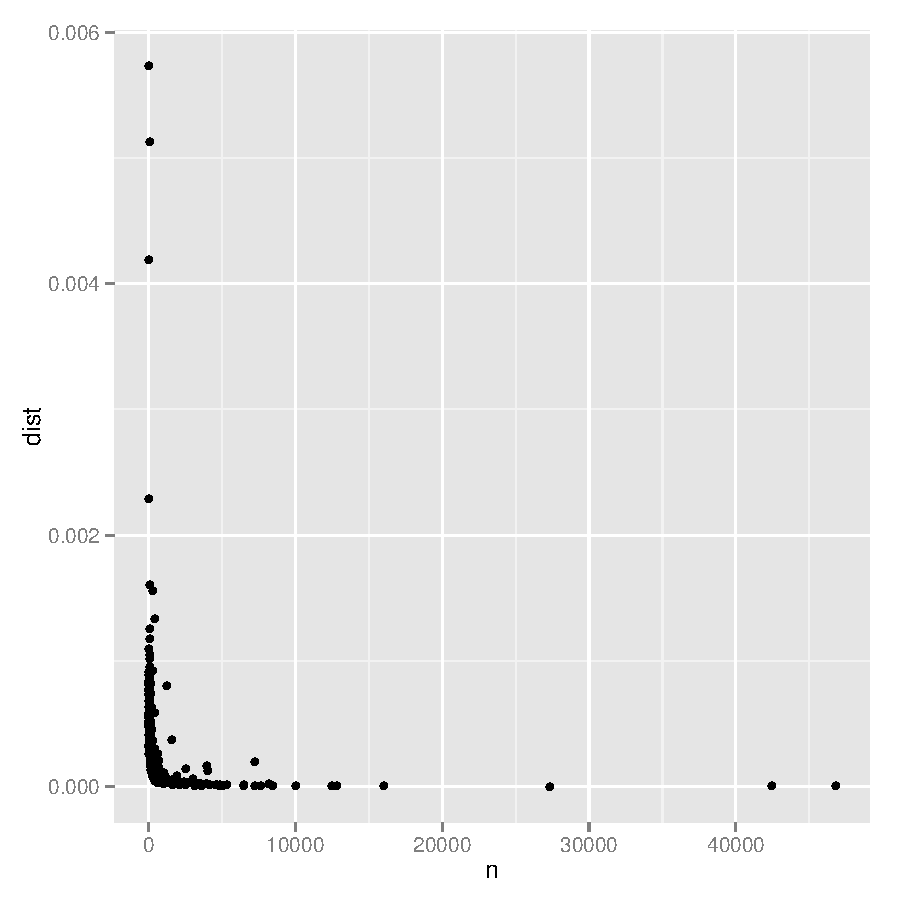
\includegraphics[width=0.5\linewidth]{case-study/n-dist-raw.pdf}
  }%
  \subfloat[Log scales]{
    \label{fig:deviation-log}
    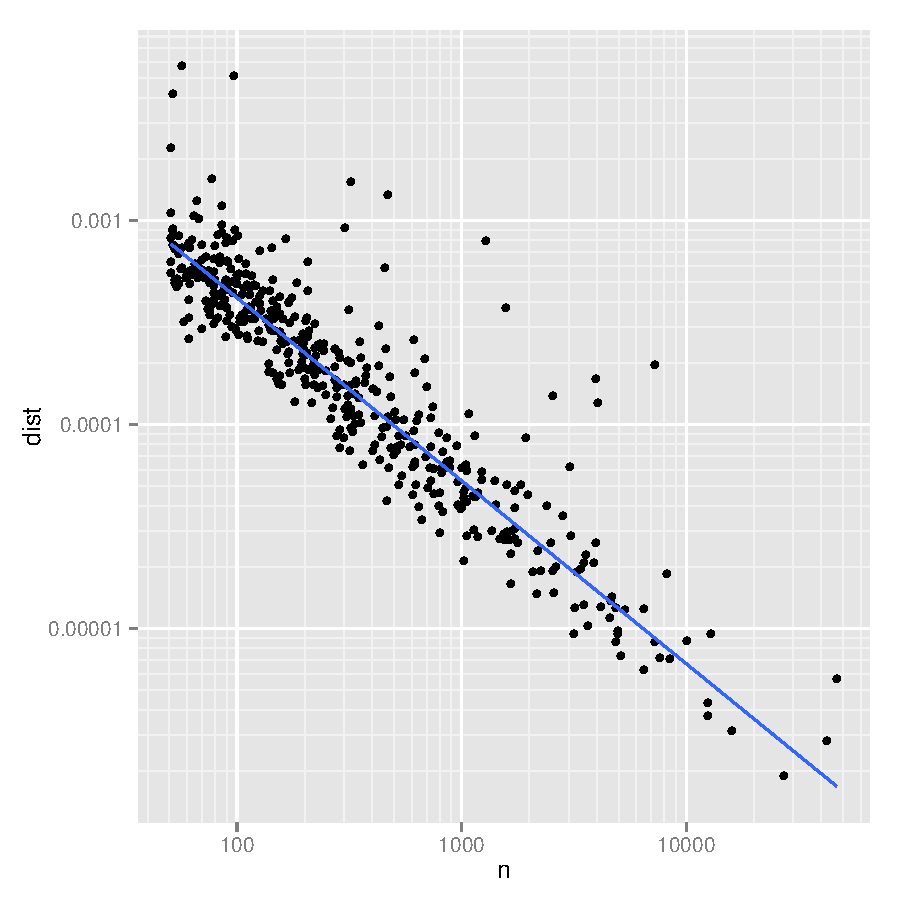
\includegraphics[width=0.5\linewidth]{case-study/n-dist-log.pdf}
  }

  \caption{(Left) Plot of n vs deviation. Variability of deviation dominated by the sample size: small samples have large variability. (Right) Log-log plot makes it easy to see pattern of variation as well as unusually high values.  Blue line is a robust line of best fit.}
  \label{fig:deviation}
\end{figure}

\begin{figure}[htbp]
  \centering
    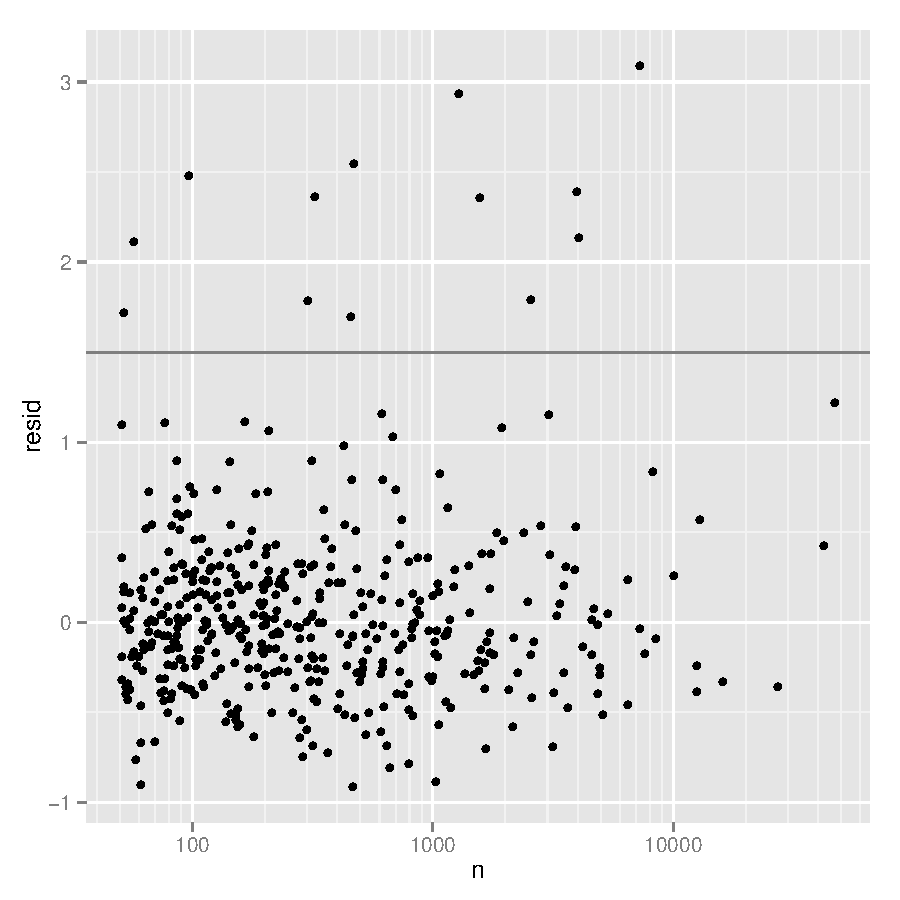
\includegraphics[width=0.5\linewidth]{case-study/n-dist-resid}
  \caption{Residuals from a robust linear model predicting $\log(dist)$ by $\log(n)$. Horizontal line at 1.5 shows threshold for further exploration.}
  \label{fig:devi-resid}
\end{figure}

We are interested in points that are high relative to other causes with the same number of deaths: these are diseases most different from the overall pattern. To find these unusual points, we fit a robust linear model and plot the residuals, as shown in Figure~\ref{fig:devi-resid}. The plot shows an empty region around a residual of 1.5, so somewhat arbitrarily we select those diseases with a residual greater than 1.5. We do that in two steps: first selecting the appropriate rows from \code{devi} (one row per disease), and then finding the matching time course information in the original summary dataset (24 rows per disease).

\begin{Verbatim}
devi$resid <- resid(rlm(log(dist) ~ log(n), data = devi))
unusual <- subset(devi, resid > 1.5)
hod_unusual <- match_df(hod2, unusual)
\end{Verbatim}

Finally, we plot the time courses of the unusual causes in Figure~\ref{fig:disease}. We break the diseases into two plots because of the differences in variability: the top plot shows diseases with over 350 deaths and the bottom with less than 350. The causes of death fall into three main groups: murders, drowning, and transportation related. Murders are more common at night, drowning in the afternoon, and transportation related during commute times. The pale gray line in the background shows the time course across all diseases.

\begin{Verbatim}
ggplot(data = subset(hod_unusual, n > 350), aes(x = hod, y = prop)) + 
  geom_line(aes(y = prop_all), data = overall, colour = "grey50") +
  geom_line() + 
  facet_wrap(~ disease, ncol = 3)
\end{Verbatim}

\begin{figure}[htbp]
  \centering
    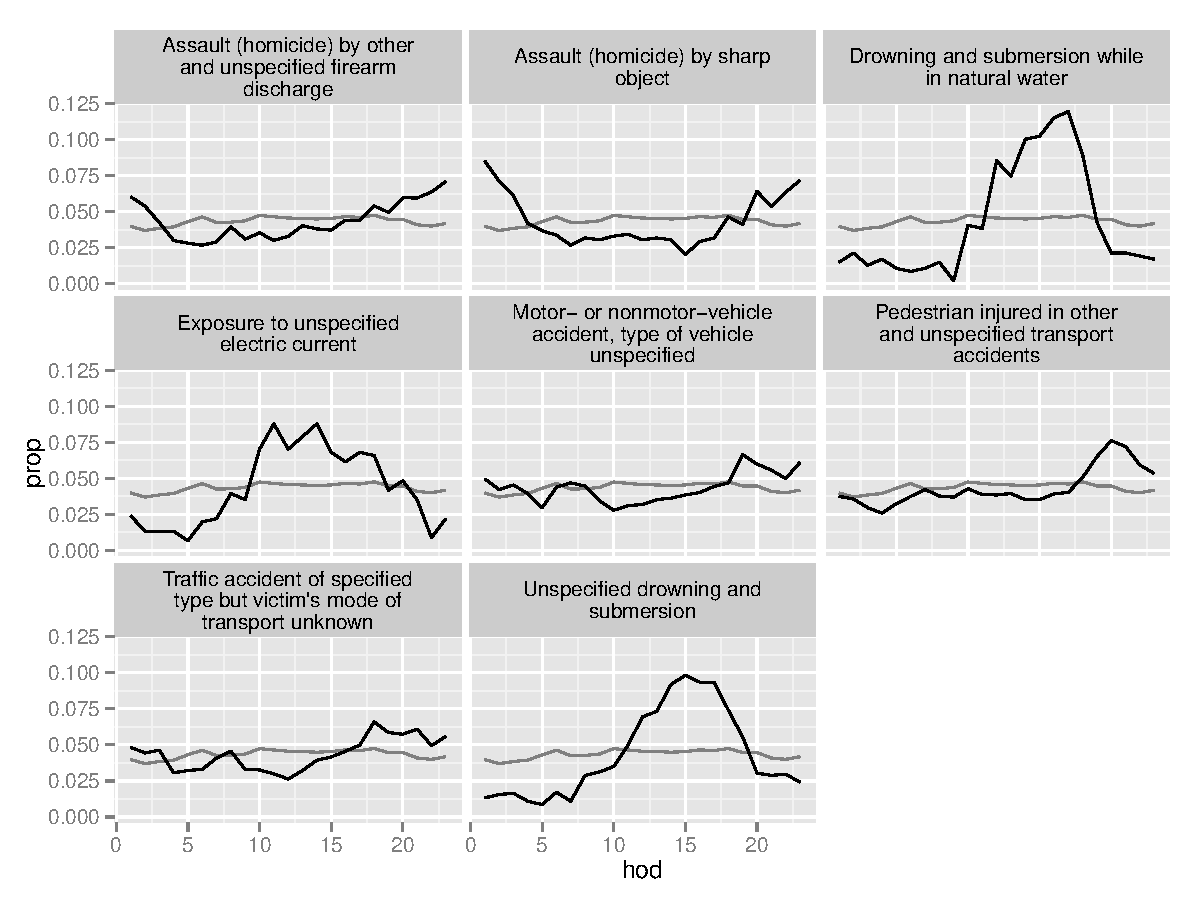
\includegraphics[width=0.9\textwidth]{case-study/unusual-big}
    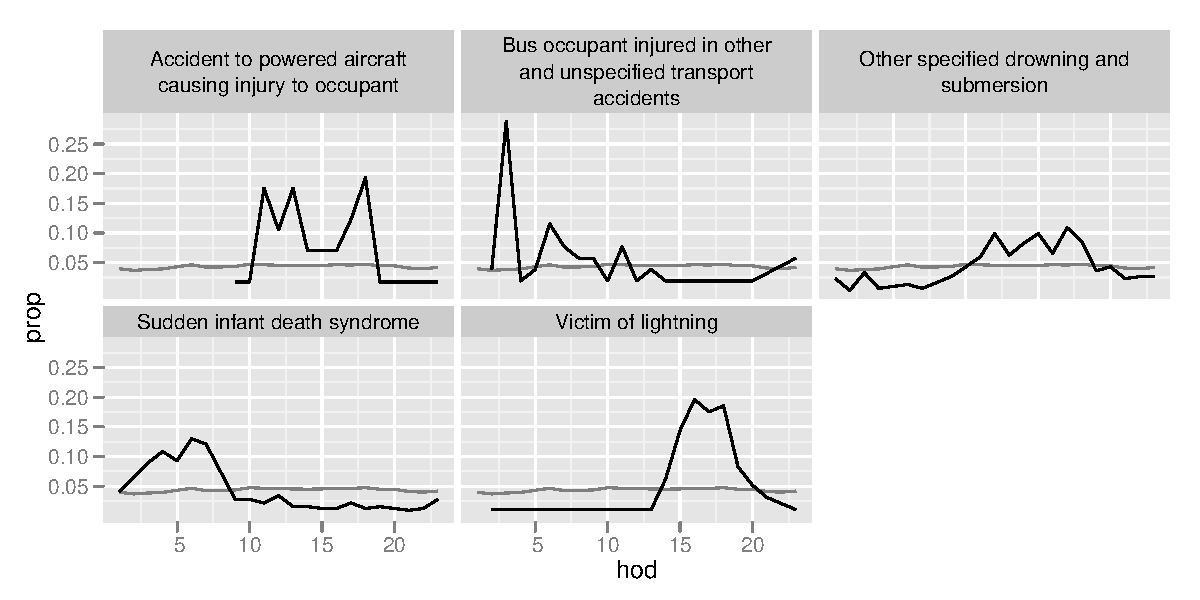
\includegraphics[width=0.9\textwidth]{case-study/unusual-sml}
  \caption{Causes of death with unusual time courses. Overall hourly death rate shown in grey. (Top) Causes of death with more than 350 deaths over a year. (Bottom) Causes of death with less than 350 deaths.  Note that different scales are used on the y axis.}
  \label{fig:disease}
\end{figure}

\section{Discussion}
\label{sec:discussion}

Data cleaning is an important problem, but it is an uncommon subject of study in statistics. This paper carves out a small but important subset of data cleaning that I've called data tidying: getting the dataset in the right structure to make further manipulation, visualisation and modelling easy. There is still much work to be done. Incremental improvements will happen as my understanding of tidy data and tidy tools improves, reducing the friction of getting data into a tidy form, and then manipulating, modelling and visualising it once it's tidy.

Bigger improvements may be possible by exploring alternative formulations of tidiness. There is a chicken-and-egg problem with tidy data: if tidy data is only as useful as the tools that work with it, then tidy tools are inextricably linked to tidy data. This makes it easy to get stuck in a local maxima where independently changing data structures or data tools does not result in an improved workflow. Breaking out of this local maxima is hard, and requires long-term concerted effort with many false starts. While I hope that this framework for tidy data is not a false start, equally, I don't see it as the final solution and I hope others will build on this framework to develop even better ways of storing data and better tools for working with it.

I have found few principles to guide the design of tidy data, which must acknowledge both statistical and cognitive factors. To date, my work has been driven by my experience doing data analysis, connections to relational database design, and introspection on the tools of data analysis. The human factors, user-centred design, and human-computer interaction communities may be able to add to this conversation, but the design of data and tools to work with it has not been an active research topic. In the future, I hope to apply methodologies from these fields (user-testing, ethnography, talk-aloud protocols) to my work to build a better understanding of the cognitive side of data analysis, and a better knowledge of how we can design tools to support the process.

Other formulations of tidy data are possible. For example, it would be possible to construct a set of tools for dealing with values stored in multidimensional arrays. This is a common data storage format for large biomedical datasets such as microarray or fMRI data. It is also necessary for many multivariate methods whose underlying theory is based on matrix manipulation. This array-tidy format would be compact and efficient, because there are many efficient tools for working with high-dimensional arrays, even when sparse, and the format would connect more closely with the mathematical basis of statistics. This approach is taken by the Pandas python data analysis library \citep{mckinney:2010}. Even more interestingly, we could consider tidy tools that can ignore the underlying data representation, automatically choosing between array-tidy and dataframe-tidy formats to optimise memory usage and performance.

Apart from tidying, there are many other tasks involved in cleaning data: parsing dates and numbers, identifying missing values, correcting character encodings (for international data), matching similar but not identical values (created by typos), verifying experimental design, and filling in structural missing values, not to mention model-based data cleaning that identifies suspicious values. Can we develop other frameworks to make these tasks easier?

% While the tools that power this work grew out of my personal struggle to work with data, the framework that hooks them all together did not develop until I had to teach data cleaning. I could look at a dataset and intuit what needed to be done to it, but I couldn't explain what I was doing, and I found it very difficult to teach. This description of tidy data in this paper easier to teach because students are pretty good at identifying variables and values, and then there is a straightforward path to follow to get data in the right format.

\section{Acknowledgements} 
\label{sec:acknowledgements}

This work wouldn't be possible without the many conversations I've had about data and how to deal with it statistically. I'd particularly like to thank Phil Dixon, Di Cook, and Heike Hofmann, who have put up with numerous questions over the years. I'd also like to thank the users of the \pkg{reshape} package who have provided many challenging problems, and my students who continue to challenge me to explain what I know in a way that they can understand. I'd also like to thank Bob Muenchen, Burt Gunter, Nick Horton and Garrett Grolemund who gave detailed comments on earlier drafts, and to particularly thank Ross Gayler who provided the nice example of the challenges of defining what a variable is and Ben Bolker who showed me the natural equivalent between a paired t-test and a mixed effects model.

% bibtool -x tidy-data.aux -c > references.bib 
\bibliography{references}

\end{document}
